\chapter{Исследовательская часть}

В данном разделе будут приведены примеры работы программы, а также проведен сравнительный анализ алгоритмов при различных ситуациях на основе полученных данных.

\section{Технические характеристики}

Технические характеристики устройства, на котором выполнялось тестирование представлены далее:
\begin{itemize}[label={---}]
	\item операционная система: Windows 11, x64;
	\item оперативная память: 8 Гб;
	\item процессор: AMD Ryzen 5 5500U с видеокартой Radeon Graphics 2.10~ГГц~\cite{amd};
	\item 6 физических ядер, 12 логических ядер~\cite{amd}.
\end{itemize}

Во время замеров времени ноутбук был нагружен только встроенными приложениями окружения.

\section{Демонстрация работы программы}

На рисунках~\ref{img:demPosl}--\ref{img:demPar} представлены результаты работы программы.

\begin{figure}[H]
	\center{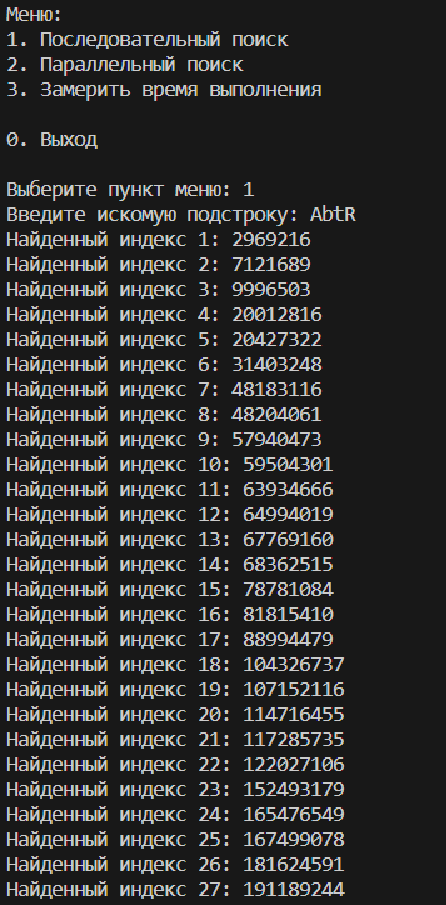
\includegraphics[width=0.3\textwidth]{img/demPosl}}
	\caption{Демонстрация работы программы (последовательный поиск)}
	\label{img:demPosl}
\end{figure}

\begin{figure}[H]
	\center{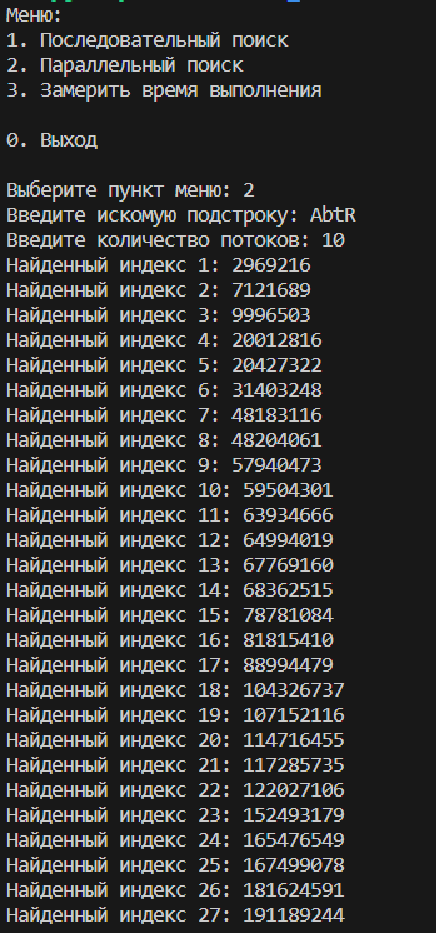
\includegraphics[width=0.3\textwidth]{img/demPar}}
	\caption{Демонстрация работы программы (параллельный поиск)}
	\label{img:demPar}
\end{figure}

\section{Время выполнения алгоритмов}

Как было сказано выше, используется функция замера процессорного времени $std::chrono::system\_clock::now()$. Функция возвращает пользовательское процессорное время типа \textit{float}.

Использовать функцию приходится дважды, затем из конечного времени нужно вычесть начальное, чтобы получить результат.

Замеры проводились для количества потоков: $$\{1, 2, 4, 8, 16, 24, 32, 40, 48, 56, 64, 72, 80, 88, 96\}$$ по 100 раз.

Результаты замеров приведены в таблице~\ref{tbl:time_mes} (время в мс).

\begin{table}[H]
	\begin{center}
		\begin{threeparttable}
			\captionsetup{justification=raggedright, singlelinecheck=off}
			\caption{Результаты замеров времени}
			\label{tbl:time_mes}
			\begin{tabular}{|c|r|}
				\hline
				Количество потоков & Время, мс \\ \hline
				1 & 1201.250\\ \hline
				2 & 683.155\\ \hline
				4 & 443.653\\ \hline
				8 & 279.936\\ \hline
				16 & 235.230\\ \hline
				24 & 228.121\\ \hline
				32 & 216.056\\ \hline
				40 & 224.693\\ \hline
				48 & 233.493\\ \hline
				56 & 225.752\\ \hline
				64 & 242.985\\ \hline
				72 & 237.691\\ \hline
				80 & 225.717\\ \hline
				88 & 244.182\\ \hline
				96 & 221.405\\ \hline
				
			\end{tabular}
		\end{threeparttable}
	\end{center}
\end{table}

По результатам замеров 32 потока является оптимальным количеством.

В таблице \ref{tbl:time_mes2} приведены результаты замеров времени для последовательной и параллельной реализаций алгоритма Кнута~---~Морриса~---~Пратта для различных длин строк. В параллельной реализации использовались 32~потока.

\begin{table}[H]
	\begin{center}
		\begin{threeparttable}
			\captionsetup{justification=raggedright, singlelinecheck=off}
			\caption{Результаты замеров времени}
			\label{tbl:time_mes2}
			\begin{tabular}{|r|r|r|}
				\hline
				Длина строки & \begin{tabular}{c}
					Последовательная\\реализация, мс
				\end{tabular} & \begin{tabular}{c}
				Параллельная\\реализация, мс
				\end{tabular} \\ \hline
				100 000 & 0.512 & 3.522\\ \hline
				200 000 & 0.946 & 3.509\\ \hline
				300 000 & 1.377 & 3.488\\ \hline
				400 000 & 1.864 & 3.582\\ \hline
				500 000 & 2.322 & 3.556\\ \hline
				600 000 & 2.729 & 3.467\\ \hline
				700 000 & 3.219 & 3.435\\ \hline
				800 000 & 3.621 & 3.521\\ \hline
				900 000 & 4.065 & 3.572\\ \hline
				1 000 000 & 4.533 & 3.435\\ \hline
				1 100 000 & 4.964 & 3.517\\ \hline
				1 200 000 & 5.434 & 3.635\\ \hline
				1 300 000 & 5.883 & 3.809\\ \hline
				1 400 000 & 6.378 & 3.915\\ \hline
				1 500 000 & 6.718 & 3.681\\ \hline
				1 600 000 & 7.198 & 3.913\\ \hline
				1 700 000 & 7.594 & 3.858\\ \hline
				1 800 000 & 8.138 & 4.041\\ \hline
				1 900 000 & 8.625 & 4.120\\ \hline
				2 000 000 & 8.943 & 4.005\\ \hline
			\end{tabular}
		\end{threeparttable}
	\end{center}
\end{table}


На рисунке~\ref{img:graph} приведена визуализация результатов замеров.

\inputPdf{graph}{Визуализация результатов замеров}


\section{Вывод}

Как видно из графика \ref{img:graph}, время выполнения последовательной реализации линейно зависит от длины исходной строки, а время выполнения параллельной реализации не зависит.
Также видно, что при длине исходной строки менее 800 000 последовательная реализация будет работать быстрее параллельной.
